\section{Electrons and Muons}
\label{sec:leptons}

Electrons and muons, being charged particles, leave identifiable tracks
within the ID.
As a result, their reconstruction involves the use of the tracks and
vertices described in the previous section, using them essentially as initial
seeds for their complete reconstruction.
Electron reconstruction, described in Section~\ref{sec:electrons}, complements the track information provided by the ID
with calorimetric information provided by the EM calorimeter (Section~\ref{sec:calo_em})
and with knowledge about the pattern of transition radiation expected to occur
in the TRT as a result of passing electrons.
Muon reconstruction, described in Section~\ref{sec:muons}, revolves around stitching together the tracks reconstructed
in the ID with those tracks independently reconstructed in the MS layers at large radii.

\subsection{Electrons}
\label{sec:electrons}

\subsubsection{Electron Reconstruction}
\label{sec:electron_reco}

The reconstruction of electron candidates is based on three components which
characterise the signature of electrons: localised clusters of energy
deposits found within the EM calorimeter, charged-particle tracks
identified in the ID, close-matching (in ($\eta,\phi$)) of the tracks to the clusters
that form the final electron candidates~\cite{Aad:2019tso}.
It is generally possible to match multiple tracks to the same electrogmagnetic cluster,
all originating from the same primary electron produced in the hard-scatter.
This is due to the fact that electrons lose significant amounts of energy to bremsstrahlung
photons as they interact with and traverse the ID.
These radiated photons can then undergo conversion to electron-positron pairs,
which, too, can undergo further bremsstrahlung.
The positrons, electrons, and photons are usually emitted in a very collimated fashion
and thus deposit most of their energy in a localised fashion within the calorimter.

The search for localised energy deposits in the EM calorimeter is performed
by following a sliding window algorithm over the individual cells whose dimensions are
defined by the second sampling layer of the EM calorimeter (Figure~\ref{fig:em_calo_section}).
Electron candidates are seeded by localised energy deposits whose summed transverse energy,
across all layers of the EM calorimeter, is greater than $2.5\,\GeV$~\cite{Aad:2019tso}.
These clusters act as seeds for the matching of reconstructed ID tracks.
The reconstructed tracks are refit using a Gaussian Sum Filter (GSF) method~\cite{ATLAS-CONF-2012-047} 
that accurately accounts for the bremsstrahlung energy losses characteristic of
electron traversal and are then matched to the localised clusters using
the cluster barycenter as the point of reference to match in $\eta-\phi$.
If there is no GSF-track candidate matching to the EM calorimeter cluster seed, then
the cluster is marked as an unconverted photon. The cluster is marked as a
converted photon if a matched GSF-track candidate exists but is not associated
with the primary hard-scatter vertex.

\subsubsection{Electron Identification}
\label{sec:electron_id}

Once electron candidates are reconstructed, they are selected based on various
levels of identification.
A further set of identification criteria is required on top of the reconstruction
so as to improve the selection of true electrons originating from the primary hard-scatter
vertex --- so-called \textit{prompt} electrons --- over \textit{non-prompt} sources
of reconstructed electrons such as those originating from photon conversions or the misidentifiation
of charged pions that leave electron-like tracks in the ID.
This identification criteria is based on the construction of a multivariate likelihood (LH) and
is referred to as the \textit{electron likelihood identification}.
The inputs to the LH are listed in Table~\ref{tab:egamma_lh_inputs} and include measurements from the tracking system in the ID,
calorimetric information, and quantities that combine the tracking and calorimetric information~\cite{Aad:2019tso}.

\begin{figure}[!htb]
    \begin{center}
        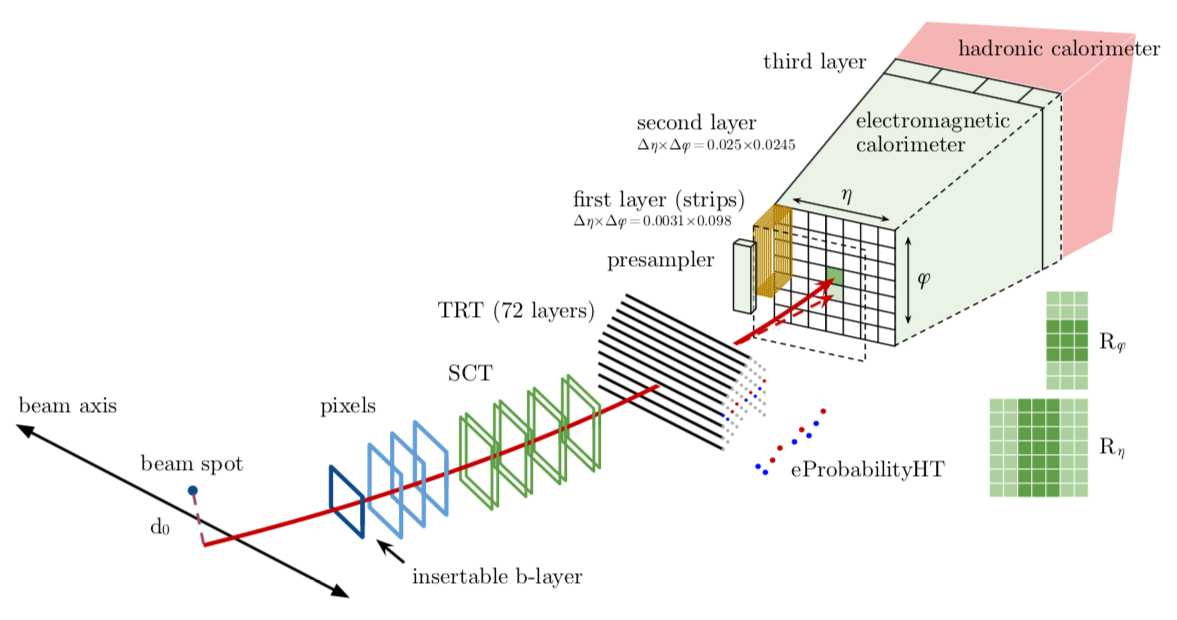
\includegraphics[width=0.9\textwidth]{figures/chapter3/egamma/egamma_lh_input_desc}
        \caption{
        }
        \label{fig:egamma_lh_input_desc}
    \end{center}
\end{figure}

The electron LH is based on the products for the signal and background probability density
functions (PDFs) associated with the set of inputs in Table~\ref{tab:egamma_lh_inputs}:

\begin{align}
    L_{S\,(B)}(\mathbf{x}) = \prod\limits_{i=1}^n P_{S\,(B),i} (x_i),
    \label{eq:egamma_lh}
\end{align}
where $\mathbf{x}$ is the vector of quantities listed in Table~\ref{tab:egamma_lh_inputs} and
the $P_{S\,(B),i}(x_i)$ are the values of the PDF for quantity $i$ at value $x_i$ for the
signal ($S$) and background ($B$).
The likelihoods are built using simulation and the signal is composed of prompt electrons
and the background is built from a combination of jets that mimic the signature of
prompt electrons, electrons from photon conversions, and non-prompt electrons from the decay
of hadrons containing heavy-flavours~\cite{Aad:2019tso}.
The final electron LH discriminant, shown in Figure~\ref{fig:egamma_lh_discriminant}, is based on a transformed version of the ratio,
\begin{align}
    d_L = \frac{L_S}{L_S + L_B},
    \label{eq:egamma_lh_disc}
\end{align}
where the transformation acts to spread $d_L$ to values not bounded by $0$ and $1$,
motivated by the need to have well-defined working points based on selections on $d_L$.

There are four such fixed values of the final LH discriminant that are used to define
four working points corresponding to increasing thresholds on the final LH discriminant:
\textsc{VeryLoose}, \textsc{Loose}, \textsc{Medium}, and \textsc{Tight}.
The efficiencies to identifiy prompt electron candidates are measured using samples of $Z\rightarrow ee$ and
$J/\psi \rightarrow ee$ following a tag-and-probe approach.
They are found, for electron candidates with $E_T > 40\,\GeV$,
to be 93\%, 88\%, and 80\% for the \textsc{Loose}, \textsc{Medium}, and \textsc{Tight} working points, respectively~\cite{Aad:2019tso}.

\begin{figure}[!htb]
    \begin{center}
    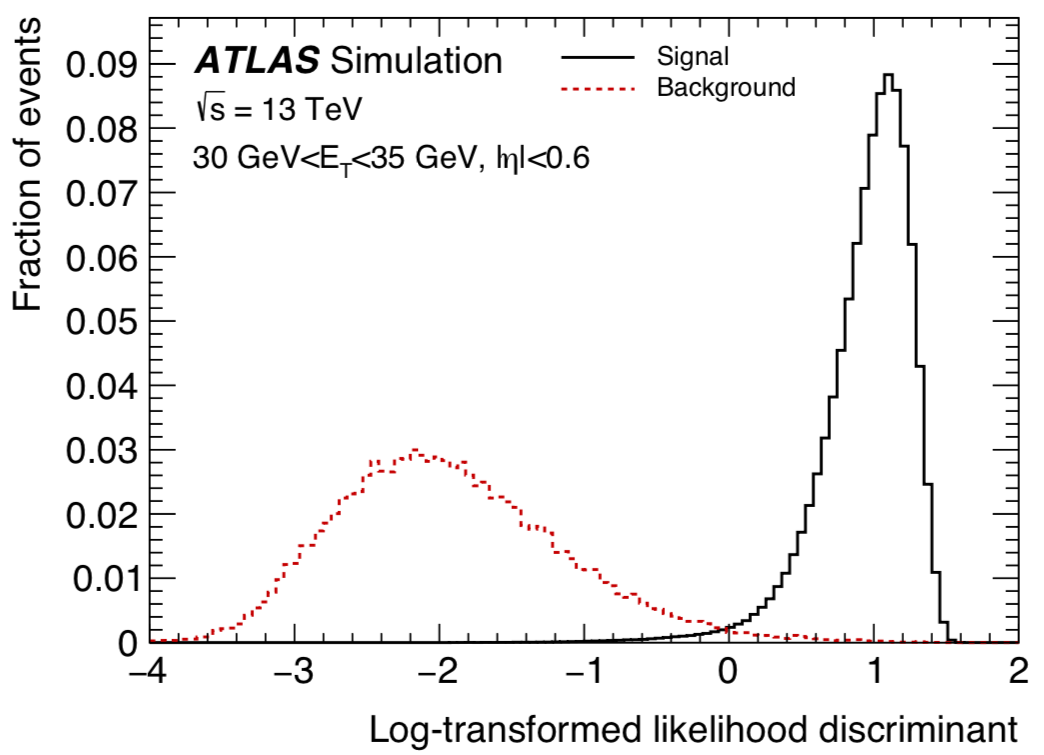
\includegraphics[width=0.7\textwidth]{figures/chapter3/egamma/egamma_lh_discriminant}
    \caption{
        Transformed LH-based electron identification discrimiant for electron candidates
        with $30\,\GeV < E_T < 35\,\GeV$ and $\lvert \eta \rvert < 0.6$.
        From Ref.~\cite{Aad:2019tso}.
    }
    \label{fig:egamma_lh_discriminant}
    \end{center}
\end{figure}

\begin{table}[!htb]
    \caption{
        Variables used as input to construct the electron identification likelihood.
        From Ref.~\cite{Aad:2019tso}.
    }
    \label{tab:egamma_lh_inputs}
    \begin{scriptsize}
    \begin{center}
    \begin{tabularx}{\textwidth}{|X|l|X|}
    \hline
    \hline
    \textbf{Input Type} & \textbf{Name} & \textbf{Description} \\
    \hline
    \multirow{2}{*}{Hadronic Leakage} & $R_{\text{had1}}$ & Ratio of $E_T$ in the first layer of the hadronic calorimeter to $E_T$ of the EM cluster \\
    \cline{2-3}
                & $R_{\text{had}}$ & Ratio of $E_T$ in the hadronic calorimeter to $E_T$ of the EM cluster \\
    \hline
    \multirow{1}{*}{Third layer of EM calorimeter} & $f_3$ & Ratio of the energy in the third layer to the total energy in the
            EM calorimeter. Only used for $E_T<30\,\GeV$  and $\lvert \eta \rvert \le 2.37$. \\
    \hline
    \multirow{3}{*}{Second layer of EM calorimter} & $w_{\eta 2}$ & Lateral shower width,
            \begin{small}$\sqrt{(\sum E_i \eta_i^2) / (\sum E_i) - ((\sum E_i \eta_i) / (\sum E_i))^2}$\end{small},
            where $E_i$ is the energy and $\eta_i$ is the pseudorapidity of cell $i$ and the sum
            is calculated within a window of $3\times5$ cells centered at the electron cluster position. \\ \cline{2-3}
            & $R_{\phi}$ & Ratio of the energy in $3\times 3$ cells over the energy in $3\times7$ cells
            centered at the electron cluster position. \\ \cline{2-3}
            & $R_{\eta}$ & Ratio of the energy in $3\times 7$ cells over the energy in $7\times7$ cells
            centered at the electron cluster position. \\ \cline{2-3}
    \hline
    \multirow{3}{*}{First layer of EM calorimeter} & $w_{stot}$ & Shower width,
            \begin{small} $\sqrt{ (\sum E_i(i - i_{\text{max}})^2)/(\sum E_i)}$ \end{small}, where $i$ runs
            over all strips in a window of $\Delta \eta \times \Delta \phi \approx 0.0625 \times 0.2$,
            corresponding typically to 20 strips in $\eta$, and $i_{\text{max}}$ is the index of the
            highest-energy strip. Used only for $E_T > 150\,\GeV$.\\ \cline{2-3}
            & $E_{\text{ratio}}$ & Ratio of the energy difference between the maximum energy deposit and the energy deposit
            in a secondary maximum in the cluster to the sum of these energies. \\ \cline{2-3}
            & $f_1$ & Ratio of the energy in the first layer to the total energy in the EM calorimeter.\\
    \hline
    \multirow{6}{*}{Track conditions} & $n_{\text{Blayer}}$ & Number of hits in the innermost pixel layer. \\ \cline{2-3}
            & $n_{\text{Pixel}}$ & Number of hits in the pixel detector. \\ \cline{2-3}
            & $n_{\text{Si}}$ & Total number of hits in the pixel and SCT detectors.\\ \cline{2-3}
            & $d_0$ & Transverse impact parameter relative to the beam-spot. \\ \cline{2-3}
            & $\lvert d_0 / \sigma(d_0) \rvert$ & Significance of transverse impact parameter defined as
            the ratio of $d_0$ to its uncertainty. \\ \cline{2-3}
            & $\Delta p / p$ &  Momentum lost by the track between the perigee and the last measurement point
            divided by the momentum at perigee. \\
    \hline
    \multirow{1}{*}{TRT} & eProbabilityHT & Likelihood probability based on transition radiation in the TRT. \\
    \hline
    \multirow{3}{*}{Track-cluster matching} & $\Delta \eta_1$  & $\Delta \eta$ between the cluster position in the first layer
            and the extrapolated track. \\ \cline{2-3}
            & $\Delta \phi_{\text{res}}$ & $\Delta \phi$ between the cluster position in the second layer of the EM calorimeter
            and the momentum-rescaled track, extrapolated from the perigee, times the charge $q$. \\ \cline{2-3}
            & $E/p$ & Ratio of the cluster energy to the track momentum. Used for $E_T>150\,\GeV$.\\
    \hline
    \hline
    \end{tabularx}
    \end{center}
    \end{scriptsize}
\end{table}

\FloatBarrier

\subsection{Muons}
\label{sec:muons}
